\documentclass[tikz,border=3pt]{standalone}
\usepackage{tikz}
\usepackage{xcolor}
\usepackage{inconsolata} % optional

\begin{document}
	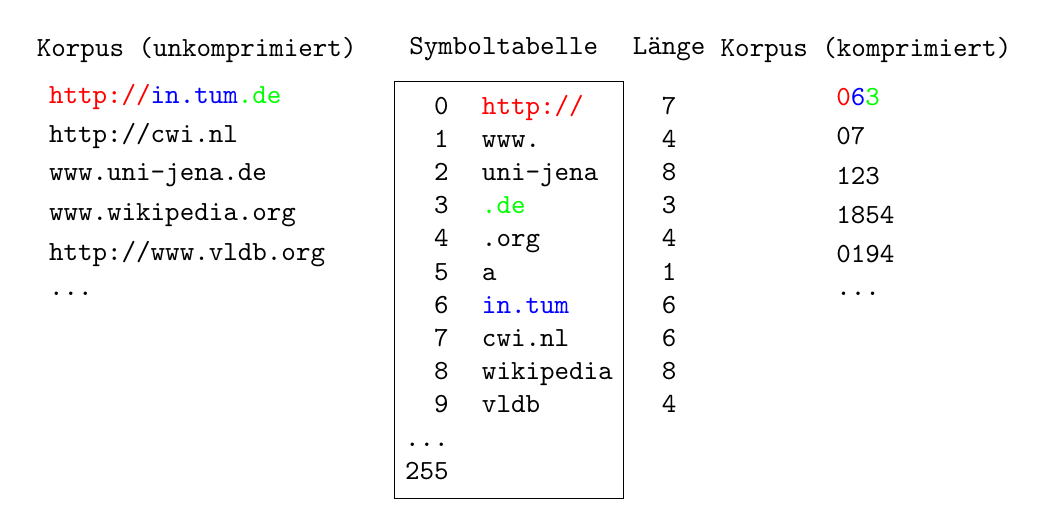
\begin{tikzpicture}[font=\ttfamily]
		
		% Linke Spalte
		\node at (0,0) {\textbf{Korpus (unkomprimiert)}};
		\node[anchor=west] at (-2,-0.6) {\textcolor{red}{http://}\textcolor{blue}{in.tum}\textcolor{green}{.de}};
		\node[anchor=west] at (-2,-1.1) {http://cwi.nl};
		\node[anchor=west] at (-2 ,-1.6) {www.uni-jena.de};
		\node[anchor=west] at (-2,-2.1) {www.wikipedia.org};
		\node[anchor=west] at (-2,-2.6) {http://www.vldb.org};
		\node[anchor=west] at (-2,-3.1) {...};
		
		% Symboltabelle
		\node at (3.9,0) {\textbf{Symboltabelle}};
		\node[draw, rectangle, anchor=north west, inner xsep=-2pt] at (2.5,-0.4) {
			\begin{tabular}{r l}
				0 & \textcolor{red}{http://} \\
				1 & www. \\
				2 & uni-jena \\
				3 & \textcolor{green}{.de} \\
				4 & .org \\
				5 & a \\
				6 & \textcolor{blue}{in.tum} \\
				7 & cwi.nl \\
				8 & wikipedia \\
				9 & vldb \\
				... \\
				255
			\end{tabular}
		};
		
		% Längen
		\node at (6,0) {\textbf{Länge}};
		\node[anchor=north] at (6,-0.4) {
			\begin{tabular}{r}
				7\\4\\8\\3\\4\\1\\6\\6\\8\\4
			\end{tabular}
		};
		
		% Rechte Spalte
		\node at (8.5,0) {\textbf{Korpus (komprimiert)}};
		\node[anchor=west] at (8,-0.6) {\textcolor{red}{0}\textcolor{blue}{6}\textcolor{green}{3}};
		\node[anchor=west] at (8,-1.1) {07};
		\node[anchor=west] at (8,-1.6) {123};
		\node[anchor=west] at (8,-2.1) {1854};
		\node[anchor=west] at (8,-2.6) {0194};
		\node[anchor=west] at (8,-3.1) {...};
		
	\end{tikzpicture}
\end{document}
